\chapter{Аналитический раздел}
\label{cha:analysis}

В данном разделе будет определена теоретическая база, необходимая для реализации поставленных задач.

\section{Описание задачи}

Дадим определение произведения двух матриц. Пусть даны прямоугольные матрицы $A$ и $B$. Размеры этих матриц $n\times{}r$ и $r\times{}m$ соответственно. Тогда результатом умножения матрицы $A$ на матрицу $B$ называется такая матрица $C$ размера $n\times{}m$, что:
\begin{equation}
    c_{ij} = \sum\limits_{k=1}^r(a_{ik}\cdot{}b_{kj})
\end{equation}
где $i = \overline{1, n}$, $j = \overline{1, m}$.

Также важно заметить, что вычисление каждого нового элемента результирующей матрицы не влияет на вычисление следующих, то есть каждый элемент матрицы считается отдельно. Значит, можно произвести распараллеливание вычислений и, тем самым, ускорить их.

\subsection{Алгоритм Винограда}
Данный алгоритм представляет собой альтернативный способ умножения матриц, позволяющий уменьшить количество операций умножения при вычислениях.

В качестве примера рассмотрим два вектора длинной 4: $U = (u_1, u_2, u_3, u_4)$ и $V = (v_1, v_2, v_3, v_4)$. Их скалярное произведение равно:
\begin{equation}
    U\times{}V = u_1\cdot{}v_1 + u_2\cdot{}v_2 + u_3\cdot{}v_3 + u_3\cdot{}v_4
\end{equation}
Левую часть этого равенства можно записать в виде:
\begin{equation}
    (u_1 + v_2)\cdot{}(u_2 + v_1) + (u_3 + v_4)\cdot{}(u_4 + v_3) - u_1\cdot{}u_2 - u_3\cdot{}u_4 - v_1\cdot{}v_2 - v_3\cdot{}v_4
\end{equation}
Это выражение допускает предварительную обработку в случае умножения двух матриц. Для каждой строки можно вычислить выражение:
\begin{equation}
    u_1\cdot{}u_2 + u_3\cdot{}u_4
\end{equation}
А для каждого столбца:
\begin{equation}
    v_1\cdot{}v_2 + v_3\cdot{}v_4
\end{equation}
Таким образом, выходит, что над заранее обработанными данными необходимо выполнить лишь 2 умножения, 5 сложений и 2 вычитания. Данная логика применима и для общего случая умножения матриц.

\subsection{Конвейеризация}
Конвейеризация – это техника, в результате которой  задача или  команда разбивается  на некоторое число подзадач, которые  выполняются последовательно. Каждая  подкоманда   выполняется на своем логическом  устройстве.    Все     логические    устройства   (ступени)  соединяются последовательно таким образом, что выход  $i$-ой   ступени   связан   с   входом   $(i+1)$-ой   ступени,  все ступени  работают  одновременно.  Множество  ступеней называется    конвейером.    Выигрыш     во    времени достигается при  выполнении  нескольких задач  за  счет параллельной   работы   ступеней,  вовлекая  на  каждом такте новую задачу или команду \cite{Conveer}.

В конвейере различают $r$ последовательных этапов, так что когда $i$-я операция
проходит $s$-й этап, то $(i+k)$-я операция проходит $(s-k)$-й этап.

\begin{figure}[H]
    \center{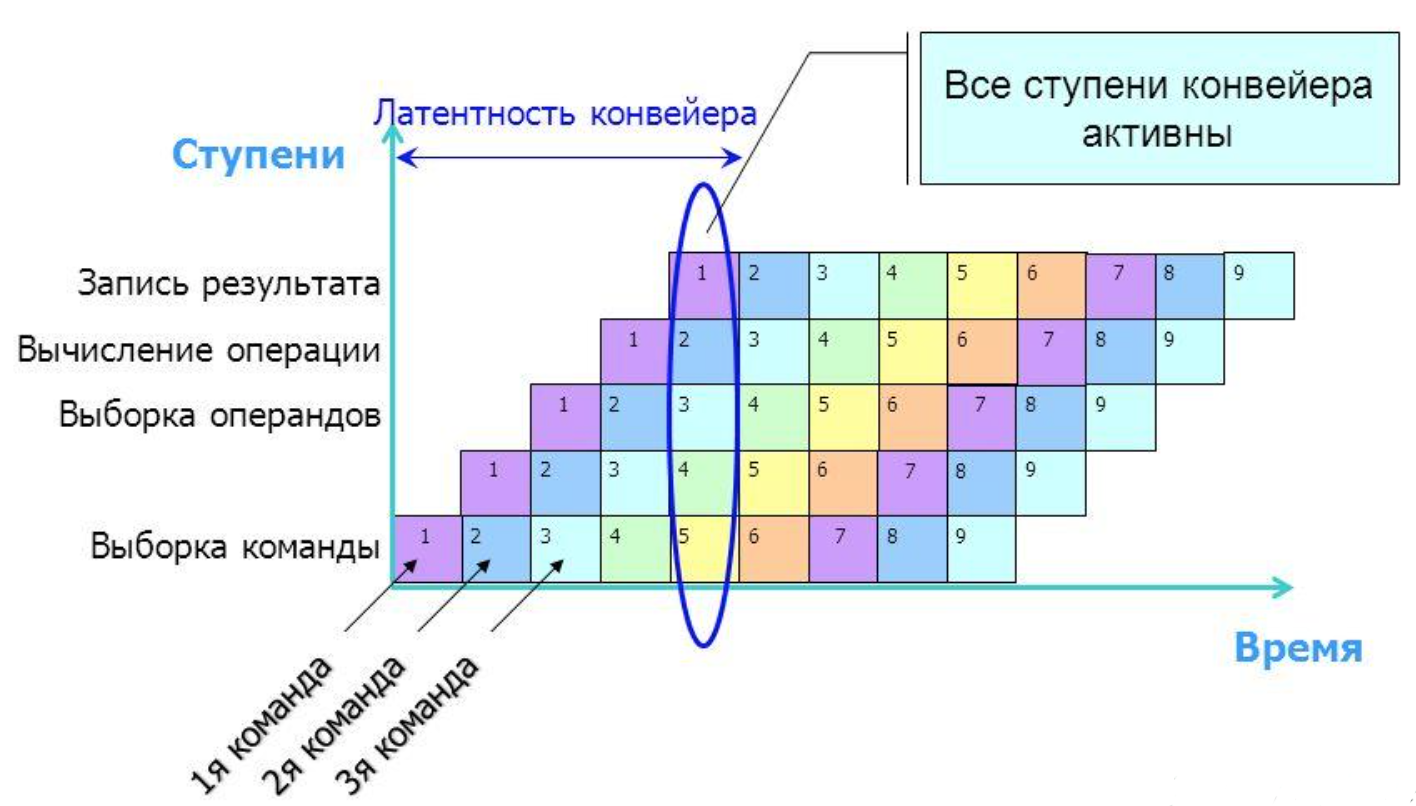
\includegraphics[scale=0.4]{./images/conveer_img.png}}
    \caption{Работа конвейра}
    \label{img:conveer}
\end{figure}

\section{Вывод}
Умножение матриц необходимый инструмент, для которого есть пути ускорения вычислений за счет уменьшения доли умножения и конвейеризации вычислений.

